\documentclass[../../main.tex]{subfiles}
\begin{document}

\subsection*{3.3}
Tra due superfici sferiche concentriche di raggio $R_1 = 10\ cm$ e $R_2 = 20\ cm$ è distribuita una carica elettrica con densità uniforme $\rho = 26.58 * 10^{-8}\ \frac{C}{m^3}$.
\\Determinare l'espressione del campo elettrostatico E(r) in funzione della distanza r dal centro del sistema.
\\Se un elettrone viene abbandonato sulla superfice esterna, quanto tempo impiega ad attraversare la cavità interna?
\\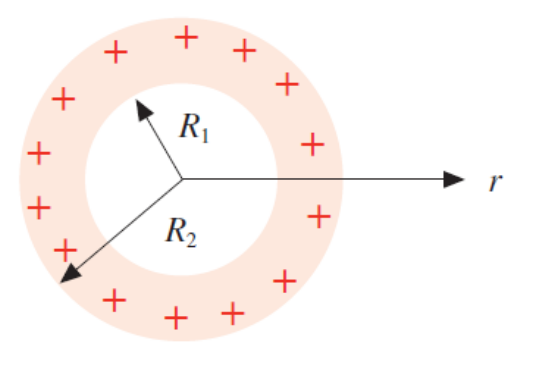
\includegraphics[scale=0.3]{e_3_3.png}
\subsubsection*{Formule utilizzate}
\subsubsection*{Soluzione punto a}
Dividiamo il problema in 3 regioni:
\\I: $o<r \le R_1$
\\II: $R_1 \le r \le R_2$
\\III: $r \ge R_2$
\\\\Regione I: $o<r \le R_1$
\\E = 0
\\\\Regione II: $R_1 \le r \le R_2$
\\$\Phi(E) = E * 4\pi r^2 = \frac{q}{\epsilon_0}$
\\$q = \int\rho dv = \rho\int dv = \rho\int_{R_1}^r 4\pi r^2dr = \rho\left[\frac{4}{3}\pi r^3\right]_{R_1}^r =\rho\frac{4}{3}\pi(r^3 - R_1^3)$
\\$E= \rho \frac{r^3-R_1^3}{3\epsilon_0 r^2}$
\\\\Regione III: $r \ge R_2$
\\$q = \rho\frac{4}{3}\pi(R_2^3-R_1^3)$
\\$E=\frac{q}{4\pi \epsilon_0 r^2} = \rho\frac{R_2^3 -R_1^3}{3\epsilon_0 r^2}$  
\subsubsection*{Soluzione punto b}
$\Delta V= V(R_1) - V(R_2) = \int_{R_1}^{R_2} E(r)dr = \frac{\rho}{3\epsilon_0}(r- \frac{R_1^3}{r^2})dr = \frac{\rho}{3\epsilon_0}\left[\frac{R_2^2 - R_1^2}{2} + R_1^3\left(\frac{1}{R_2} - \frac{1}{R_1}\right)\right] = 100V$
\\$E_k = 100\ eV = 1.6 * 10^{-17}\ J$
\\$v = \sqrt{\frac{2E_k}{m_e}} = \sqrt{\frac{2 * 1.6 * 10^{-17}}{9.1 * 10^{-31}}} = 5.93 * 10^6\ \frac{m}{s}$
\\$t = \frac{l}{v} = \frac{2R_1}{v} = \frac{0.2}{5.93 * 10^6} = 33.7\ nS$
\newpage

\end{document}